\chapter{Background}
\label{ch:background}

\section{LSB Reacting Flow Field}

This section will discuss the salient features of the LSB flow field that will play an important part in the discussions to follow in this thesis.

As discussed in Section \ref{subsec:literature-review-lsb}, there have been multiple variations of the LSB design used by researchers in the past.
Broadly, they can be classified into jet-LSB and vane-LSB, based on the means used to produce the weak swirl in the flow field.
This study reports findings relating to the vane-LSB design, and hence, our discussion will also pertain to the vane-LSB.

\begin{figure}

\centering

\begin{tikzpicture}

\draw [thin, dashed] ( -3, 0 ) -- ++( 11, 0 );
\draw [thin, dashed] ( 0, -2.5 ) -- ++( 0, 5 );

% Top view
% Perforated plate
\draw [red] ( 0, 0 ) circle ( 2.6416/2 );

\draw [red] ( 0, 0 ) circle ( 0.28194/2 );
\foreach \theta in { 0, 45, ..., 360 }
  \draw [red] ( \theta : 0.508 ) circle ( 0.28194/2 );
\foreach \theta in { 0, 22.5, ..., 360 }
  \draw [red] ( \theta : 0.9525 ) circle ( 0.28321/2 );

% Outer edge
\draw ( 0, 0 ) circle ( 3.8/2 );
\draw ( 0, 0 ) circle ( 1.85 );

% Vanes
\foreach \theta in { 0, 22.5, ..., 360 } {
  \draw [blue] ( \theta - 2.5 : 1.3208 ) -- ( \theta - 2.5 : 1.85 );
  \draw [blue] ( \theta + 2.5 : 1.3208 ) -- ( \theta + 2.5 : 1.85 );
}

% Side View
% Inner edge
\draw ( 5 - 1.9, -1.3208 ) rectangle ++( 3.8, 2.6416 );
\draw [pattern = north west lines] ( 5 - 1.9, -1.3208 ) rectangle ++( 3.8, 0.05 );
\draw [pattern = north west lines] ( 5 - 1.9, 1.3208 ) rectangle ++( 3.8, -0.05 );

% Outer edge
\draw [pattern = north west lines] ( 5 - 1.3208, 1.9 ) rectangle ++( 2.6416, -0.05 );
\draw ( 5 - 1.3208, 1.85 ) rectangle ++( 2.6416, -1.85 + 1.3208 );
\draw [pattern = north west lines] ( 5 - 1.3208, -1.9 ) rectangle ++( 2.6416, 0.05 );
\draw ( 5 - 1.3208, -1.85 ) rectangle ++( 2.6416, 1.85 - 1.3208 );

% Vanes
\draw [blue] ( 4, -1.85 ) rectangle ++( 2, 1.85 - 1.3208 );
\draw [blue] ( 4, 1.85 ) rectangle ++( 2, -1.85 + 1.3208 );

% Perforated plate
\draw [red] ( 5 - 1.9, -1.3208 ) rectangle ++( -0.127, 2.6416 );
\draw [red, pattern = north east lines, pattern color=red] ( 5 - 1.9, -1.3208 ) rectangle ++( -0.127, 0.226695 );
\draw [red, pattern = north east lines, pattern color=red] ( 5 - 1.9, -0.810895 ) rectangle ++( -0.127, 0.161925 );
\draw [red, pattern = north east lines, pattern color=red] ( 5 - 1.9, -0.14097 ) rectangle ++( -0.127, -0.22606 );
\draw [red, pattern = north east lines, pattern color=red] ( 5 - 1.9, 0.14097 ) rectangle ++( -0.127, 0.22606 );
\draw [red, pattern = north east lines, pattern color=red] ( 5 - 1.9, 0.810895 ) rectangle ++( -0.127, -0.161925 );
\draw [red, pattern = north east lines, pattern color=red] ( 5 - 1.9, 1.3208 ) rectangle ++( -0.127, -0.226695 );

\end{tikzpicture}

\caption[Schematic of a vaned swirler]{The figure shows a top and side cross-sectional view of the vaned swirler design used in this study. The perforated plate used to control the relative mass flow split is highlighted in \textcolor{red}{red}, while the vanes used to generate swirl are highlighted in \textcolor{blue}{blue}.}

\label{fig:swirler}

\end{figure}



The vane-LSB---or simply \emph{LSB} from here on---uses a vaned swirler
with a central open section.
A typical design of such a swirler is shown in Figure \ref{fig:swirler}.
The swirler splits the flow into two streams, imparting swirl only to the outer annular flow.
A perforated plate covers the open central section of the swirler and controls the relative mass flow split between the central unswirled flow and the annular swirling flow.
The swirler is located at the head of a constant area nozzle which abruptly expands into the combustion zone.

\subsection{Role of swirl and recirculation zones}

The amount of swirl present in the resulting flow is characterized by a theoretical swirl number, \(S\), which represents the ratio of angular momentum to axial momentum in the flow field.
Cheng et al.\cite{2000-cheng} and later, Littlejohn et al.\cite{2002-littlejohn} reduced this to the following equation.

\begin{equation}
S = \frac{2}{3} \tan \alpha \frac{ 1 - R^3 }{ 1 - R^2 + \left[ M^2\left( \dfrac{1}{R^2} - 1 \right)^2 \right]R^2}
\label{eqn:theoreticalSwirlNumber}
\end{equation}

In Equation \ref{eqn:theoreticalSwirlNumber}, \(R\) is the ratio of the diameter of the central section to the outer diameter of the swirler.
Similarly, \(M\) is the ratio of the mass flow rate through the central portion to the mass flow rate through the outer (vaned) portion of the swirler.
Finally, \(\alpha\) is the angle of the vanes of the swirler.

Along with the recess length of the swirler, the theoretical swirl number was identified to be a key parameter that determines the LSB operating regime.\cite{2002-littlejohn}
Typical values of \(S\) in low swirl combustion range from 0.4--0.6.

\begin{figure}

\centering

\begin{tikzpicture}

% Nozzle
\draw[pattern=north east lines] ( 0, 0.8 ) -- ++( 1.15, -0.3 ) -- ++( 1.85, 0 ) -- ++( 0, 1.025 ) -- ++( -0.05, 0 ) -- ++( 0, 0.05 ) -- ++( 0.05, 0 ) -- ++( 0, 0.025 ) -- ++ ( -0.1, 0 ) -- ++( 0, -0.6 ) -- ++( -2.9, 0 ) -- cycle;
\draw[pattern=north east lines] ( 0, -0.8 ) -- ++( 1.15, 0.3 ) -- ++( 1.85, 0 ) -- ++( 0, -1.025 ) -- ++( -0.05, 0 ) -- ++( 0, -0.05 ) -- ++( 0.05, 0 ) -- ++( 0, -0.025 ) -- ++ ( -0.1, 0 ) -- ++( 0, 0.6 ) -- ++( -2.9, 0 ) -- cycle;
\draw ( 0, 0.8 ) -- ++( 0, -1.6 );
\draw ( 3, 0.5 ) -- ++( 0, -1 );

% Swirler
\draw ( 1.15, 0.5 ) -- ++( 0.7, 0 ) -- ++( -0.7, -0.15 ) -- ++( 0.7, 0 ) -- ++( -0.7, 0.15 ); 
\draw ( 1.15, 0.5 ) -- ++( 0, -0.15 );
\draw ( 1.85, 0.5 ) -- ++( 0, -0.15 );
\draw ( 1, 0.35 ) rectangle ++( 1, -0.7 );
\draw ( 1.15, -0.5 ) -- ++( 0.7, 0 ) -- ++( -0.7, 0.15 ) -- ++( 0.7, 0 ) -- ++( -0.7, -0.15 ); 
\draw ( 1.15, -0.5 ) -- ++( 0, 0.15 );
\draw ( 1.85, -0.5 ) -- ++( 0, 0.15 );
\draw [pattern = horizontal lines] ( 0.95, 0.35 ) rectangle ++( 0.05, -0.7 );

% Quartz tube
\draw [fill = blue!10!white] ( 2.95, 1.525 ) rectangle ++( 8.05, 0.05 );
\draw [fill = blue!10!white] ( 2.95, -1.525 ) rectangle ++( 8.05, -0.05 );
\draw ( 11, 1.525 ) -- ++( 0, -3.05 );

% Centerline
\draw [dashed, thin] ( -1, 0 ) -- ++( 13, 0 );

% TRZ
\draw [blue, very thick, ->] ( 4, 1 ) arc ( 0 : 275 : 0.25 ) -- ++( 0.2, 0 );
\draw [blue, very thick, ->] ( 4, -1 ) arc ( 0 : -275 : 0.25 ) -- ++( 0.2, 0 );

% CRZ
\draw [blue, very thick, ->] ( 5.5, 0.5 ) arc ( 180 : 90 : 0.5 ) .. controls +( 0.5, 0 ) and +( 0.5, 0 ) .. ++( 0, -0.5 ) -- ++( -0.2, 0 );
\draw [blue, very thick, ->] ( 5.5, -0.5 ) arc ( 180 : 270 : 0.5 ) .. controls +( 0.5, 0 ) and +( 0.5, 0 ) .. ++( 0, 0.5 ) -- ++( -0.2, 0 );

\node at ( 3.75, 0 ) {TRZ};
\node at ( 6, 0 ) {CRZ};

\end{tikzpicture}

\caption[Location of recirculation zones in the LSB flow field]{The figure shows the locations of the recirculation zones in the LSB flow field. The Toroidal Recirculation Zone (TRZ) forms near the abrupt area expansion. The Central Recirculation Zone (CRZ) forms within a recirculation bubble along the centerline of the combustor.}

\label{fig:recirculationZones}

\end{figure}



Figure \ref{fig:recirculationZones} shows the locations of the notable recirculation zones in the LSB flow field.
The toroidal recirculation zone forms near the inlet, while the central recirculation zone forms within a recirculation bubble along the centerline.
In conventional swirl combustion, the function of the swirl is to induce these recirculation zones that help stabilize the flame by causing a feedback of heat and radicals from the products into the reactants.
In particular, the toroidal recirculation zone traps hot combustion products and continually ignites the reactants at the base of the flame.\cite{2005-johnson}

In the LSB flow field, these recirculation zones are not only much weaker, but also, do not play any part in the stabilization of the flame.
Instead, the LSB flame is a freely propagating turbulent flame that is stabilized by the divergent flow coming from the inlet nozzle.
The function of the swirl in the LSB flow field is merely to enhance this divergence.
This purely aerodynamic means of stabilizing the flame differentiates the LSB regime from conventional swirl combustion.

\subsection{Axial velocity profile and self-similarity}
\label{subsec:lsb-axial-velocity-profile}

The mean axial velocity profile along the centerline of the LSB exhibits a characteristic linear profile in the near field of the inlet.
Two features can be associated with this profile.
First, extrapolating the velocity profile to the point upstream where the axial velocity equals the reference velocity, we obtain the location of the virtual origin.
The virtual origin represents the point upstream where the divergence seemingly originates from.
Second, we can measure the slope of the linear region of the axial velocity profile and obtain the axial stretch rate.

Cheng et al.\cite{2006-cheng,2008-cheng-a} investigated these two parameters using a non-preheated setup at atmospheric pressure.
They found that the virtual origin for reacting LSB flow fields asymptotically decreases at low/moderate Reynolds numbers, while the mean axial stretch rate is nearly independent of the same parameter.
This means that at moderately increasing Reynolds numbers, the divergent flow structure shifts upstream into the injector, eventually ceasing this motion for high Reynolds number values (above 70,000).

Since this shift does not affect the slope of the velocity profile, the researchers plotted the mean axial velocity profiles for different operating conditions, shifted to have a common virtual origin.
Further, the velocity profiles were normalized by the mass-averaged inlet velocity (called the reference velocity).
The resultant plot showed that the linear section of the divergent flow was self-similar at all the velocities tested.
This self-similarity of the mean axial velocity profile was used to explain other observations regarding the flame characteristics which we will discuss shortly.

\subsection{Flame stabilization mechanism}
\label{subsec:lsb-flame-stabilization-mechanism}

The flame stabilization mechanism in the LSB is purely aerodynamic.
The turbulent flame is not anchored in the sense of an attached flame, but freely propagates into the reactants.
Conventionally, attached flames are preferred in combustion systems as lifted flames are associated with unstable/undesirable characteristics like blow off.
However, the LSB flame is robustly stabilized and not prone to blow off.

The location where the LSB flame is stabilized is marked by the equilibrium condition for flame stabilization---the local reactant velocity, \(U\) equals the local turbulent flame propagation velocity, \(S_T\).
The decrease in the local reactant velocity along the centerline of the combustor is accompanied by an increase in the local turbulence level.
In other words, along the axis of the combustor, at the location where the flame is stabilized, the reactant velocity is decreasing, while the turbulent flame propagation velocity (which scales with the local turbulence) is increasing.

This sets up a stable equilibrium for the flame.
Small perturbations causing the flame to move upstream are offset by the increased reactant velocity, while similar perturbations downstream are counteracted by the increased turbulent flame speed.
This is the mechanism behind the robust stabilization of the LSB flame.

\subsection{Effect of Flow Parameters on Flame Characteristics}

The operating conditions of the LSB combustor are fully described by four fundamental flow parameters; the combustor pressure, \(p\), the combustor temperature, \(T\), the mixture equivalence ratio, \(\phi\), and the reference velocity, \(U_0\).
The reference velocity represents the mass-averaged velocity of the reactants entering the LSB and is defined after Cheng et al.\cite{2000-cheng} as follows.

\begin{equation}
U_0 = \frac{ \left( \dfrac{ \dot{m}_{air} }{ \rho_{air} } \right) + \left( \dfrac{ \dot{m}_{fuel} }{ \rho_{fuel} }\right) }{ \dfrac{\pi d_s^2 }{4} }
\label{eqn:referenceVelocity}
\end{equation}

In this section, we will discuss the effect each of these flow parameters has on the location and shape of the LSB flame.

\subsubsection{Reference Velocity}

As described earlier in Section \ref{subsec:lsb-flame-stabilization-mechanism}, the LSB flame is stabilized where the local reactant velocity and turbulent flame speed are equal.

Unlike the laminar flame speed, \(S_L\), the turbulent flame speed is not uniquely determined by the reactant composition and thermodynamic conditions.
Instead, it is a function of the flow characteristics and the burner geometry as well.

A simple model proposed by Damk{\"o}hler\cite{1996-glassman} treats the turbulent flame as a wrinkled laminar flame.
The presence of these wrinkles vastly increases the surface area of the flame, increasing the rate at which the reactants can be consumed through the flame.
The size of these wrinkles can be related to the rms of the local reactant velocity, \(u'\).
Expressed mathematically, this leads to Equation \ref{eqn:damkohlerModel}.

\begin{equation}
\frac{ S_T }{ S_L } = 1 + \frac{ u' }{ S_L }
\label{eqn:damkohlerModel}
\end{equation}

Cheng et al.\cite{2002-cheng,2009-cheng,2010-littlejohn} observed that the slope of this linear relationship was dependent on the fuel mixture being used.
This idea is encapsulated in Equation \ref{eqn:chengModel} that presents a modified version of Equation \ref{eqn:damkohlerModel}.

\begin{equation}
\frac{ S_T }{ S_L } = 1 + K \frac{ u' }{ S_L }
\label{eqn:chengModel}
\end{equation}

The constant \(K\) has a value of around 1.73 for methane-air mixtures and a somewhat higher value---3.15---for hydrogen-air mixtures,\cite{2009-cheng} suggesting that the turbulent flame speed is affected strongly by the thermo-diffusive properties of the fuel.

In order to predict the expected effect of increasing the reference velocity, consider the following analysis at the flame standoff location where \(U\)=\(S_T\).

\begin{align}
\frac{ S_T }{ S_L } &= 1 + K \frac{ u' }{ S_L } \nonumber \\
S_T &= S_L + K u' \nonumber \\
\implies U &= S_L + K u' \nonumber \\
U_0 - \frac{ dU }{ dx } ( X_f - X_0 ) &= S_L + K u' \nonumber \\
\therefore X_f &= X_0 + \frac{1 - \left( \dfrac{ S_L }{ U_0 } + K\dfrac{ u' }{ U_0 } \right) }{ \dfrac{ dU }{ dx } }
\label{eqn:flameImmobility}
\end{align}

Consider the terms on the RHS of Equation \ref{eqn:flameImmobility}.
As discussed in Section \ref{subsec:lsb-axial-velocity-profile}, the virtual origin location is invariant for moderate to high values of reference velocity.
In the same section, we also discussed how the slope of the velocity profile, \(\dfrac{ dU }{ dx }\), is also invariant with reference velocity.
In the numerator of the second term, the local turbulence intensity, \(\dfrac{ u' }{ U_0 }\), can also be expected to be a constant, since \(u'\) should scale with the reference velocity in the same manner as long as the burner geometry doesn't change.
That leaves only the term \(\dfrac{ S_L }{ U_0 }\) as a function of \(U_0\).
Typically, the laminar flame speeds are an order of magnitude lower (\(\approx O(1)\) m/s) than the reference velocities at which the LSBs are operated (\(\approx O(10)\) m/s).
As a result, this term is vanishingly small, leaving the RHS independent of \(U_0\).
In other words, the flame location, \(X_f\) is expected to be invariant with the reference velocity at which the LSB is operated.

% Flame angle
% Flame structure

\subsubsection{Preheat Temperature}

\subsubsection{Swirler Vane Angle}

\subsubsection{Equivalence Ratio}

\subsubsection{Combustor Pressure}

\section{CH PLIF Signal Modeling}
\label{sec:background-chplif-signal-modeling}

While the intent and scope of this work is to use CH PLIF as a visualization technique to image the flame front with high fidelity, it would be extremely useful to be able to predict the CH PLIF signal intensity for different reactant mixtures and initial conditions as a means to gauge the feasibility of applying the technique to acquire high fidelity images of the flame at those conditions.
To that end, this discussion will attempt to develop a mathematical model to calculate, in a semi-quantitative manner, the rate of CH PLIF photons emitted by the illuminated reaction zone.
The following discussion introduces important concepts in LIF signal intensity calculation using a simple two-level model and then proceeds to apply these concepts to model the more complicated physical processes in the CH system.

\subsection{Basic Model}
\label{subsec:chplif-basic-model}

In its most basic form, the number of fluorescence photons generated in a system, \(\Phi\) is the product of the number of emitters, \(N\) and the Einstein coefficient for spontaneous emission, \(A\).

\begin{equation}
  \Phi = N\times A
  \label{eqn:fluorescencePhotons}
\end{equation}

The fluorescence photons produced are radiated in all directions and only a fraction of these can be recorded by a collection system in an experiment.
This fraction is determined by the experimental set up, the collection angle, and the efficiency of the optics and the detector used to record the signal.
For this analysis, however, this fraction is omitted to reduce complexity.

\begin{figure}

\centering

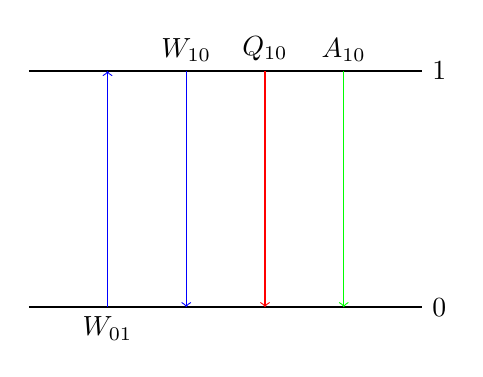
\begin{tikzpicture}

% Lower state
\draw [thick] ( 0, 0 ) -- ++( 5, 0 );

% Upper state
\draw [thick] ( 0, 3 ) -- ++( 5, 0 );

% Transitions
\draw [blue, ->] ( 1, 0 ) -- ++( 0, 3 );
\draw [blue, ->] ( 2, 3 ) -- ++( 0, -3 );
\draw [red, ->] ( 3, 3 ) -- ++( 0, -3 );
\draw [green, ->] ( 4, 3 ) -- ++( 0, -3 );

\node at ( 5, 0 ) [right] {0};
\node at ( 5, 3 ) [right] {1};

\node at ( 1, 0 ) [below] {\(W_{01}\)};
\node at ( 2, 3 ) [above] {\(W_{10}\)};
\node at ( 3, 3 ) [above] {\(Q_{10}\)};
\node at ( 4, 3 ) [above] {\(A_{10}\)};

\end{tikzpicture}

\caption[Transitions in a basic two-level model for fluorescence]{The figure shows energy levels and transitions between two levels, labeled 0 and 1, in a basic model of laser-induced fluorescence. Stimulated absorption and emission are shown in \textcolor{blue}{blue}, collisional quenching is shown in \textcolor{red}{red} and spontaneous emission is shown in \textcolor{green}{green}.}

\label{fig:twoLevel}

\end{figure}



In a simple two-level model for the fluorescing system, as shown in Figure \ref{fig:twoLevel}, Equation \ref{eqn:fluorescencePhotons} may be expanded in terms of the number density of the emitters, \(n\), and the volume in which the fluorescence occurs, \(V\).

\begin{equation}
  \Phi = n_1VA_{10}
\end{equation}

The population of the upper state, \(n_1\) can be solved for by rate analysis.
The mathematical treatment is not particularly complicated and is covered in detail by various textbooks and review papers.\cite{1996-eckbreth,1997-daily}
Here, we shall merely remark that the functional form of the solution has two limiting cases.
The limits are decided by the relative magnitudes of the pumping rate, \(W_{01}\), and the relaxation rate given by the sum of the spontaneous emission rate and the collisional quenching rate, \(A_{10} + Q_{10}\).
The former is the rate at which the upper energy level is populated through absorption.
The latter represents the rate at which the molecules return to the lower energy state, either through spontaneous emission or by losing energy to other molecules through inelastic collisions.

When the pumping rate is far lower compared to the relaxation processes (\(W_{01}\ll A_{10}+Q_{10}\)), the solution tends to the weak excitation limit.
In this limit, the functional form of the solution is shown in Equation \ref{eqn:twoLevelModel-weak}

\begin{equation}
  \Phi = n_0 V W_{01}\overbrace{\frac{A_{10}}{A_{10}+Q_{10}}}^{\text{Fluorescence Yield}}
  \label{eqn:twoLevelModel-weak}
\end{equation}

The \(n_0VW_{01}\) term in Equation \ref{eqn:twoLevelModel-weak} represents the number of molecules that are excited to the upper state per second, while the fluorescence yield represents the fraction of these molecules that will produce a LIF signal.
In typical combustion environments, the fluorescence yield is usually small, since the collisional quenching rate dominates the spontaneous emission rate.
The rate of collisional quenching of the marker species by another species in the flame is proportional to the frequency of collisions between the two species.
Further, the effectiveness of such collisions is decided by a collision cross-section, \(\sigma\), which is often a function of the temperature.
Equation \ref{eqn:quenchingRate} presents the calculation of the collisional quenching rate by summation over all the species, \(i\), in the flame.

\begin{align}
  Q_{10} &= \sum_i n_i \times \sigma_i \times c_i \nonumber \\
  & = \sum_i n_i \sigma_i \sqrt{\frac{8kT}{\pi\mu_i}} \nonumber \\
  & = \sqrt{\frac{8kT}{\pi}} \sum_i \frac{n_i \sigma_i}{\sqrt{\mu_i}}
  \label{eqn:quenchingRate}
\end{align}

In Equation \ref{eqn:quenchingRate}, \(k\) is the Boltzmann constant, \(T\) is the local temperature, \(n_i\) is the number density of species \(i\) and \(\mu_i\) represents the reduced mass of the colliding molecules, given by Equation \ref{eqn:reducedMass}.

\begin{equation}
  \mu_i = \frac{ m_i m }{ m_i + m }
  \label{eqn:reducedMass}
\end{equation}

In Equation \ref{eqn:reducedMass}, \(m\) is the mass of the marker species, while \(m_i\) are the masses of the colliding species.
Since LIF in combustion primarily targets minor species, by probability, these collisions will almost always occur with major species in the system.
As a result, the summation in Equation \ref{eqn:quenchingRate} need only be carried out over the major species in the flame.
The values of the local number densities of the major species can be measured by techniques like Raman scattering, or can be obtained from solving chemical kinetics models.

\subsubsection{Absorption Integral Calculation}
\label{subsubsec:basic-model-absorption-integral-calculation}

Let us now briefly examine the first term in Equation \ref{eqn:twoLevelModel-weak} in further detail.
Let \(\phi(\nu)\) represent the normalized lineshape of the absorption line being excited, such that \(\int \phi(\nu) d\nu = 1\).
If \(B_{01}\) is the Einstein coefficient for absorption for the line being excited, the term \(B_{01}\phi(\nu)\) represents the spectral absorptivity of the line at \(\nu\).
\(B_{01}\) is usually presented in m\(^2\)/Js for LIF applications.
Similarly, let \(I_\nu\) be the spectral intensity of the incident radiation, which is the intensity (power per area) of the laser beam per spectral interval.
Let \(\psi(\nu)\) be the normalized spectral profile of the laser lineshape, such that \(I_\nu\) = \(I \psi(\nu)\) and \(\int \psi(\nu) d\nu = 1\).
\(I_\nu\) is usually given in W/cm\(^2\)/cm\(^{-1}\) for ease of use in laser applications.

The product of the spectral absorptivity and the spectral intensity integrated over the spectrum, gives the pumping rate, \(W_{01}\), as shown in Equation \ref{eqn:pumpingRate-unsimplified}.
The factor \(c\) is the speed of light, which brings the units of \(W_{01}\) to s\(^{-1}\).

\begin{equation}
  W_{01} = \frac{I}{c} \int \psi(\nu) B_{01}\phi(\nu) d\nu
  \label{eqn:pumpingRate-unsimplified}
\end{equation}

\subsubsection{Population Distribution}
\label{subsubsec:basic-model-population-distribution}

Once again, consider Equation \ref{eqn:twoLevelModel-weak}, this time focusing on the term \(n_0\), the number density of the marker species in the lower energy state that are available for excitation to the upper state.
In reality, this comprises only a small subset of all the available molecules of the marker species in the system.

\begin{equation}
  n_0 = nf_0
  \label{eqn:boltzmannFraction}
\end{equation}

In Equation \ref{eqn:boltzmannFraction}, \(n\) is the number density of all marker species over all the energy levels, while the fraction, \(f_0\), represents the proportion of the marker species that populates the lower energy level.

\subsubsection{Solution}
\label{subsubsec:basic-model-solution}

Substituting Equations \ref{eqn:pumpingRate-unsimplified} and \ref{eqn:boltzmannFraction} into \ref{eqn:twoLevelModel-weak}, and noting that the signal produced is actually integrated over a volume,

\begin{equation}
  \Phi = \int_V \frac{n A_{10}}{A_{10} + Q_{10}} \frac{I}{c} f_0 B_{01} \textcolor{red}{\int_\nu \psi(\nu) \phi_j(\nu) d\nu} dV
  \label{eqn:twoLevelModel-unsimplified}
\end{equation}

In Equation \ref{eqn:twoLevelModel-unsimplified}, the absorption integral from Equation \ref{eqn:pumpingRate-unsimplified} is highlighted in \textcolor{red}{red}.
The outer integral is performed in space, over the portion of the flame illuminated by the laser sheet.
Under the assumption that the laser intensity is uniformly distributed over the sheet thickness, it is possible to rewrite the outer integral as a 1-D integral over the thickness of the flame by replacing the laser intensity, \(I\) with the laser power, \(P\).

\begin{equation}
  \Phi = \frac{P}{c} \int_x \frac{n A_{10}}{A_{10}+Q_{10}} f_0 B_{01} \int_\nu \psi(\nu) \phi_j(\nu) d\nu dx
  \label{eqn:twoLevelModel}
\end{equation}

Equation \ref{eqn:twoLevelModel} is thus, the solution to the two-level model in the weak excitation limit.
Note that the LIF signal varies linearly as the incident laser power (or intensity).
Consequently, the weak excitation limit is also referred to as the linear regime.

For the sake of completion, we will briefly mention the other limit of the two-level model solution that occurs when the rate of pumping far exceeds the relaxation rate (\(W_{01} \gg A_{10} + Q_{10}\)).
This is called the saturated limit and in this limit, the fluorescence signal ceases to change with the intensity of the incident laser beam.
Operating in this regime is generally not preferred due to several reasons.
First, the magnitude of the LIF signal per unit incident laser intensity tends to be the maximum in the linear regime.
Once the variation ceases to be linear (even before nearing the saturation limit), we get diminishing returns for increasing the laser power.
Further, the saturation criterion (maintaining a high laser intensity) is difficult to satisfy simultaneously in the spatial, temporal and spectral domains.
For these reasons, we will restrict our discussion hence forward the linear regime only.

\subsection{CH PLIF Process}
\label{subsec:background-ch-plif-process}

In this section, we will examine the limitations of trying to apply the two-level model to describe the CH PLIF process.

Laser-Induced Fluoresence is a multi-step process.
First, the marker species absorbs a photon and transitions from a lower energy state to a higher one.
This is followed by several physical processes, of which only one pathway leads to the spontaneous de-excitation of the excited molecule, accompanied by the release of a photon.
The de-excitation can---but does not need to---take the molecule back to the original state.
If the molecule does return to its original state, the fluorescence is said to be resonant.
Due to the difficulty of measuring fluorescence signals at the same wavelength as the excitation beam, most practical applications of LIF tend to be non-resonant.
The choice of the spectral and temporal properties of the excitation laser source, and of the detected fluorescence emission, constitute the excitation and detection schemes.

The excitation scheme chosen for this study follows the work done by Li et al.\cite{2007-li-a} who used a ring-cavity, pulsed alexandrite laser to provide excitation in the vicinity of the R-bandhead of the CH \(B^2\Sigma^- \leftarrow X^2\Pi\) (0,0) system.
This bandhead, shown in Figure \ref{fig:chB-XAbsorption}, is found at a wavelength of about 387.2 nm and represents transitions from a ground state rotational quantum number of \(N''=7\).
When operated in multimode, alexandrite lasers have relatively large bandwidths (a few cm\(^{-1}\) is not uncommon) and hence make it possible to excite several of the neighboring transitions near the bandhead.
The current implementation excites CH molecules in the ground state \(X^2\Pi\), \(v''=0\) with rotational quantum numbers \(N''\) between 5--9.

\begin{figure}

\centering

\input{figures/chB-XAbsorptionPlot}

\caption[CH \(B^2\Sigma^-\leftarrow X^2\Pi\) (0,0) R-bandhead absorption lines]{The figure shows the frequencies of the absorption lines near the R-bandhead of the CH \(B^2\Sigma^-\leftarrow X^2\Pi\) (0,0) band. The individual lines are labeled with corresponding \(N''\) quantum number.}

\label{fig:chB-XAbsorption}

\end{figure}



Upon excitation, these molecules transition to the second electronically excited \(B^2\Sigma^-\) state and populate the lowest vibrational level, (\(v'=0\)).
Since these transitions occur in the R-branch, the rotational quantum number increases by +1, resulting in the population of the \(N'\) levels between 6--10.
At this point, the following possibilities exist for the excited molecule:

\begin{enumerate}
  \item The molecule can undergo inelastic collisions with other molecules, resulting in relaxation in the rotational, vibrational or electronic manifolds.
  \item The molecule can spontaneously emit a photon and return to any of the lower energy states.
  \item The molecule can experience stimulated emission in the presence of another photon of the appropriate frequency and return to any of the lower energy states.
  \item The molecule can experience further excitation either by absorbing a photon or through collisional means and can react chemically.
\end{enumerate}

Now, let us examine these potential pathways in greater detail.
The first pathway pertains to relaxation.
The excitation and subsequent population of a higher energy state causes the CH population distribution to deviate from the equilibrium Boltzmann distribution.
The degree of relaxation possible is limited by the lifetime of the energy level the excited species occupy.
The collision-free, radiative lifetime of the \(B\) electronic state is about 300 ns\cite{1996-luque-c}---long enough for sufficient rotational relaxation to occur, but too short for complete vibrational relaxation.
Based on experiments conducted by Garland et al.\cite{1985-garland-b}, it is estimated that the vibrational energy transfer between the two bound states available to the \(B^2\Sigma^-\) state is about two orders of magnitude slower than the rotational energy transfer.
As a result, we may suppose that the vibrational manifold remains relatively unaffected, while the rotational manifold is relaxed closer to an equilibrium distribution.
The question of the electronic relaxation will be addressed later in this discussion.

The second option available for the excited CH molecule is to spontaneously emit a photon and return to a lower energy state.
Spontaneous de-excitation to the ground state primarily follows the diagonal \(B^2\Sigma^-\rightarrow X^2\Pi\) (0,0) band.
The rate of such spontaneous emission between two states is given by the Einstein emission coefficient for the transition.
Once again, we will defer discussion of the \(B-A\) transition until later in this discussion.

The third option is for the CH molecule to experience stimulated emission in the presence of a photon of an appropriate frequency.
It is highly unlikely that the apposite photon would have a frequency other than the excitation laser.
The rate of stimulated emission induced by the excitation laser beam is proportional to the Einstein absorption coefficient for the transition.
Other photons that can induce stimulated emission in the CH molecules could originate from spontaneous emission or CH* chemiluminescence.
As mentioned earlier, it is highly unlikely that these will result in stimulated emission of any significant proportion.
In part, this is due to the spatial distribution of CH in a typical flame.
In Chapter \ref{ch:introduction}, it was stated that CH molecules are expected to be found only in the thin reaction zone of the flame.
This causes most photons to be emitted in directions away from the flame, reducing their chance of encountering more CH molecules.
Since CH is a minor species, its concentrations are inherently too low, further reducing the likelihood of this pathway.

The fourth option is for the molecule to experience further excitation by absorbing multiple photons or through collisions with other energetic molecules in the system.
Since most available photons do not match any transitions from the \(B^2\Sigma^-\), \(v=0\) state, it is unlikely to experience multi-photon excitation.
However, collisional removal of CH molecules from the \(B\) state is certainly possible.

\begin{figure}

\centering

\input{figures/chRKRPlot}

\caption[Potential curves for the CH system]{The figure shows the RKR potential curves for the \(X^2\Pi\), \(A^2\Delta\) and \(B^2\Sigma^-\) energy levels in the CH system. A few vibrational levels are indicated for the \(X^2\Pi\) and \(A^2\Delta\) states. The \(B^2\Sigma^-\) state has only two bound vibrational levels. The diagram is reproduced from Richmond et al.\cite{2005-richmond} who based it on \emph{ab initio} calculations by van Dishoeck\cite{1987-vandishoeck}}

\label{fig:chRKR}

\end{figure}



Having listed all the options, let us resume the discussion on the possibility of electronic energy transfer from the excited \(B^2\Sigma^-\), \(v'=0\) state.
The spacing of the energy levels in the CH system, shown in Figure \ref{fig:chRKR}, is such that the \(B^2\Sigma^-\), \(v'=0\) state is found to be near-degenerate with the \(A^2\Delta\), \(v=1\) energy level.
Consequently, the \(B^2\Sigma^-\leftrightarrow A^2\Delta\) (0,1) transition is reversible.
Due to this, collisional population of the \(A^2\Delta\) \(v=0,1\) states from the \(B^2\Sigma^-\) \(v=0\) state occurs rapidly.
Garland et al.\cite{1985-garland-b} measured that these transfers account for almost a quarter of all collisional depletion of the \(B^2\Sigma^-\), \(v=0\) level.
Theoretical calculations using overlap integrals between the involved energy levels predict that a majority of these transfers will be along the diagonal (0,0) transition.\cite{2000-luque}.
Instead, experimental data indicates that the number is closer to a fifth, with almost 80\% of the transfers following the near-degenerate (0,1) pathway.

It is this electronic energy transfer mechanism that enables our excitation scheme to record high quality CH PLIF images.
Having now populated the \(A^2\Delta\) states, the resulting spontaneous emission from the \(A^2\Delta\rightarrow X^2\Pi\) (0,0) and (1,1) transitions can be easily observed between 420--440 nm.
A small portion of the fluorescence in this wavelength range also occurs from the \(B^2\Sigma^-\rightarrow X^2\Pi\), (0,1) transition.
Since these emission wavelengths are located far from the excitation wavelength, a simple glass filter is sufficient to suppress any elastic scattering from the laser beam.

\subsection{Improved Model}
\label{subsec:chplif-improved-model}

While the two-level model is conceptually simple, applying it to describe the complicated physical process of CH PLIF is challenging.
Daily\cite{1997-daily} notes, for example, that significant errors can result from using the two-level model to describe even a three-level system.
Hence, it is worthwhile to investigate a more complicated model that can describe the CH system with higher fidelity.

\begin{figure}

\centering

\begin{tikzpicture}

% Ground states
\draw [thick] ( 3, 0 ) -- ++( 4, 0 );
\node at ( 7, 0 ) [right] {\(X^2\Pi, v = 0\)};
\draw [thick] ( 3, 1 ) -- ++( 4, 0 );
\node at ( 7, 1 )  [right] {\(X^2\Pi, v = 1\)};

% First electronic states
\draw [thick] ( 0, 4 ) -- ++( 3, 0 );
\node at ( 0, 4 )  [left] {\(A^2\Delta, v = 0\)};
\draw [thick] ( 0, 5 ) -- ++( 3, 0 );
\node at ( 0, 5 )  [left] {\(A^2\Delta, v = 1\)};

% Second electronic state
\draw [thick] ( 7, 5 ) -- ++( 3, 0 );
\node at ( 10, 5 )  [right] {\(B^2\Sigma^-, v = 0\)};

% Transitions
\draw [blue, ->] ( 6, 0 ) -- ++( 3, 5 );

\draw [red, ->] ( 6.5, 5 ) -- ++( -3, 0 );
\draw [red, ->] ( 6.5, 4.75 ) -- ++( -3, -0.75 );

\draw [green, ->] ( 8, 5 ) -- ++( -2.25, -4 );
\draw [green, ->] ( 1, 4 ) -- ++( 3, -4 );
\draw [green, ->] ( 1, 5 ) -- ++( 3, -4 );

\end{tikzpicture}

\caption[Relevant transitions in a CH molecule]{Some of the important transitions between energy levels in a CH molecule are shown. The excitation of the CH molecules (\textcolor{blue}{blue}) is followed by collisional energy transfer processes (\textcolor{red}{red}) which populate additional energy levels. Spontaneous emission from some of these energy levels (\textcolor{green}{green}) is collected.}

\label{fig:energyLevels}

\end{figure}



Figure \ref{fig:energyLevels} shows the relevant pathways that lead to the fluorescence emission as discussed in Section \ref{subsec:background-ch-plif-process}.
An accurate model of the CH system should involve at least five energy levels, namely the \(B^2\Sigma^-\), \(v=0\), \(A^2\Delta\), \(v=0,1\), and \(X^2\Pi\), \(v=0,1\) levels.
The model will need to account for collisional transfers between each of these levels, in addition to spontaneous and stimulated transitions.
The mathematical solution quickly becomes tedious and complicated.
Further, it involves several rate coefficients that have not yet been measured experimentally.

Fortunately, this can be significantly simplified.
Previous studies\cite{1996-luque-c,2000-luque} have indicated that the off-diagonal \(B\rightarrow X\) (0,1) transition plays a relatively minor role accounting for only 3.5\% of the total fluorescence.
Further, the radiative \(A\rightarrow X\) transitions are known\cite{1996-luque-b} to be strongly diagonal, with little or no interaction\cite{1985-garland-b} between the two states.
The net result of these two assertions is that we can treat the two \(B\rightarrow A\rightarrow X\) pathways to be disjoint and parallel.
The resulting pseudo-three-level model is shown in Figure \ref{fig:simplifiedEnergyLevels}.

\begin{figure}

\centering

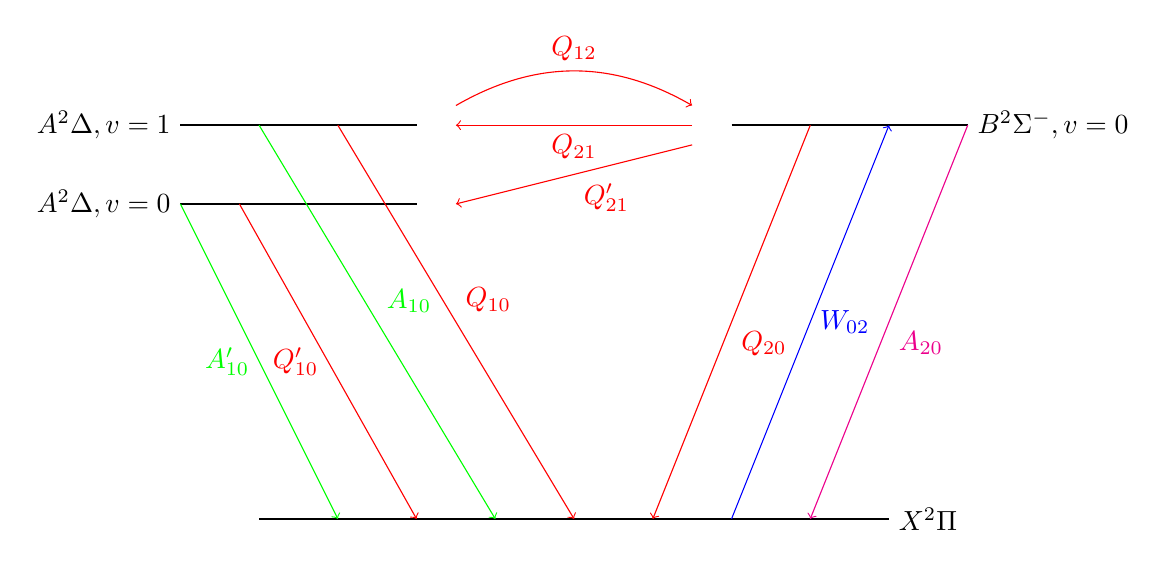
\begin{tikzpicture}

% Ground state
\draw [thick] ( 1, 0 ) -- ++( 8, 0 );
\node at ( 9, 0 ) [right] {\(X^2\Pi\)};

% First electronic states
\draw [thick] ( 0, 4 ) -- ++( 3, 0 );
\node at ( 0, 4 ) [left] {\(A^2\Delta, v = 0\)};
\draw [thick] ( 0, 5 ) -- ++( 3, 0 );
\node at ( 0, 5 ) [left] {\(A^2\Delta, v = 1\)};

% Second electronic state
\draw [thick] ( 7, 5 ) -- ++( 3, 0 );
\node at ( 10, 5 ) [right] {\(B^2\Sigma^-, v = 0\)};

% Transitions
\path [->, blue] ( 7, 0 ) edge node [right] {\(W_{02}\)} ++( 2, 5 );
\path [->, red] ( 8, 5 ) edge node [auto] {\(Q_{20}\)} ++( -2, -5 );
\path [->, magenta] ( 10, 5 ) edge node [auto] {\(A_{20}\)} ++( -2, -5 );

\path [->, red] ( 6.5, 5 ) edge node [auto] {\(Q_{21}\)} ++( -3, 0 );
\path [->, red] ( 6.5, 4.75 ) edge node [auto] {\(Q'_{21}\)} ++( -3, -0.75 );
\path [->, red] ( 3.5, 5.25 ) edge [bend left] node [above] {\(Q_{12}\)} ++( 3, 0 );

\path [->, red] ( 2, 5 ) edge node [auto] {\(Q_{10}\)} ++( 3, -5 );
\path [->, green] ( 1, 5 ) edge node [auto] {\(A_{10}\)} ++( 3, -5 );

\path [->, red] ( 0.75, 4 ) edge node [left] {\(Q'_{10}\)} ++( 2.25, -4 );
\path [->, green] ( 0, 4 ) edge node [left] {\(A'_{10}\)} ++( 2, -4 );

\end{tikzpicture}

\caption[Transitions in the improved CH fluorescence model]{A simplified model of the transitions between the energy levels in a CH system. Excitation (\textcolor{blue}{blue}) of ground state CH molecules to the upper electronic state is followed by several collisional energy transfer processes (\textcolor{red}{red}). A small portion of these molecules spontaneously emit a photon (\textcolor{green}{green}) and return to ground state. The spontaneous emission corresponding to resonant PLIF (\textcolor{magenta}{magenta}) is not collected.}

\label{fig:simplifiedEnergyLevels}

\end{figure}



According to this model, the lower state of the CH system is treated as a single pool that CH molecules are excited from and returned to.
This not only neglects the rotational manifold, but also the vibrational manifold of the ground state.
This assumption would be valid as long as most of the CH molecules occupy the \(v=0\) state and the fraction of molecules in the \(v=1\) state can be safely neglected.
At flame temperatures of about 2200 K, this assumption is somewhat questionable as only about 83\% of the ground state CH molecules occupy the \(v=0\) level and as much as 14\% are found at the \(v=1\) state.
However, in light of the simplifications afforded to our semi-quantitative model by this assumption, we retain it.

The rates of the various transition processes are indicated in Figure \ref{fig:simplifiedEnergyLevels}.
\(W_{02}\) is the pumping process that populates the \(B\)(0) state.
\(Q_{ij}\) are collisional energy transfer processes that transfer CH molecules from the \(i\) level to the \(j\) level.
The subscripts 0, 1 and 2 represent the electronic energy levels \(X\), \(A\) and \(B\).
Processes involving the \(A\)(0) state are differentiated from those involving the \(A\)(1) state by a prime (\('\)).
Finally, \(A_{ij}\) represents the spontaneous emission coefficients between the \(i\) and \(j\) levels.

Applying Equation \ref{eqn:fluorescencePhotons} to this case, we can write an expression for the LIF signal intensity as follows,

\begin{equation}
  \Phi = ( n_1 A_{10} + n'_1 A'_{10} )V
  \label{eqn:signalIntensity}
\end{equation}

Our task is to solve for the values of \(n_1\) and \(n'_1\) in terms of \(n_0\).
To do this we need to write rate equations describing the variation of the populations of the three upper states with time.

\begin{align}
  \frac{dn_1}{dt} &= -( A_{10} + Q_{10} + Q_{12} )n_1 + Q_{21} n_2
  \label{eqn:rates1}\\
  \frac{dn'_1}{dt} &= -( A'_{10} + Q'_{10} )n'_1 + Q'_{21} n_2
  \label{eqn:rates2}\\
  \frac{dn_2}{dt} &= W_{02} n_0 + Q_{12} n_1 - ( A_{20} + Q_{20} + Q_{21} + Q'_{21} )n_2
  \label{eqn:rates3}
\end{align}

Under the assumption that the laser excitation time scale is much longer that the collisional time scales, we can set the LHS of Equations \ref{eqn:rates1}--\ref{eqn:rates3} to zero.
This results in a closed set of linear equations, which can be expressed in matrix form as follows.

\begin{equation}
  \left[
    \begin{matrix}
      A_{10} + Q_{10} + Q_{12} & 0 & -Q_{21}\\
      0 & A'_{10} + Q'_{10} & -Q'_{21}\\
      -Q_{12} & 0 & A_{20} + Q_{20} + Q_{21} + Q'_{21}
    \end{matrix}
  \right]\left[
    \begin{matrix}
      n_1\\
      n'_1\\
      n_2
    \end{matrix}
  \right] = \left[
    \begin{matrix}
      0\\
      0\\
      W_{02}n_0
    \end{matrix}
  \right]
  \label{eqn:closedForm}
\end{equation}

From Equation \ref{eqn:closedForm}, we only need the solutions to \(n_1\) and \(n'_1\).
Substituting the solutions directly into Equation \ref{eqn:signalIntensity}, we can write the solution in the following form to mirror the expression in Equation \ref{eqn:twoLevelModel-weak}.

\begin{equation}
  \Phi = n_0VW_{02}(Y + Y')
  \label{eqn:improvedModel-weak}
\end{equation}

The terms \(Y\) and \(Y'\) in Equation \ref{eqn:improvedModel-weak} are non-dimensional and represent the fluorescence yields from the two \(A^2\Delta\) states.
The functional expression for the yields is more complex now, as shown in Equations \ref{eqn:fluorescenceYield1-unsimplified}--\ref{eqn:fluorescenceYield2-unsimplified}.

\begin{align}
  Y &= \frac{ Q_{21} A_{10} }{ ( A_{10} + Q_{10} + Q_{12} )( A_{20} + Q_{20} + Q_{21} + Q'_{21} ) - Q_{12}Q_{21} }
  \label{eqn:fluorescenceYield1-unsimplified}\\
  Y' &= \frac{ ( A_{10} + Q_{10} + Q_{12} )Q'_{21} A'_{10} }{ ( A'_{10} + Q'_{10} ) ( ( A_{10} + Q_{10} + Q_{12} )( A_{20} + Q_{20} + Q_{21} + Q'_{21} ) - Q_{12}Q_{21} ) }
  \label{eqn:fluorescenceYield2-unsimplified}
\end{align}

\subsubsection{Absorption Integral Calculation}
\label{subsubsec:improved-model-absorption-integral-calculation}

We now focus on the first portion of Equation \ref{eqn:improvedModel-weak} and consider the rate of population of the upper \(B^2\Sigma^-\) state.
As in case of the simple model, this term involves the computation of the integral of the product of the laser linewidth function, \(\psi(\nu)\) and the absorption linewidth function, \(\phi(\nu)\).
However, since our excitation scheme targets multiple lines in the R-bandhead, we actually have a summation of several absorption lines in this integral.

\begin{align}
  W_{02} & = \frac{I}{c} \int \psi(\nu) \sum_j B_j \phi_j (\nu) d\nu \nonumber \\
        & = \frac{I}{c} \sum_j B_j \int \psi(\nu)\phi_j(\nu) d\nu
  \label{eqn:pumpingRate}
\end{align}

In Equation \ref{eqn:pumpingRate}, the terms \(B_j\) are the absorption coefficients, \(B_{02}\), for each transition being excited, each of which has its own broadened linewidth, \(\phi_j(\nu)\) at the local conditions.
The discussion of the various sources of line broadening that need to be considered for our case is defered till Chapter \ref{ch:chplif}.

\subsubsection{Population Distribution}
\label{subsubsec:improved-model-population-distribution}

Equation \ref{eqn:boltzmannDistribution} presents the expression for \(f_j\) in terms of the vibrational and rotational quantum numbers, (\(v\), \(J\)), of the energy level \(j\).

\begin{equation}
  f_j(v,J) = \frac{ \exp{\left(\dfrac{-hcE_v(v)}{kT}\right)} (2J + 1)\exp{\left(\dfrac{-hcE_r(v, J)}{kT}\right)} }{ Q_{rv} }
  \label{eqn:boltzmannDistribution}
\end{equation}

The vibrational energy, \(E_v(v)\) of a level is calculated according to Equation \ref{eqn:vibrationalEnergy}, while the rotational energy, \(E_r(v,J)\) is calculated according to Equation \ref{eqn:rotationalEnergy}.

\begin{align}
  E_v(v) &= \omega_e \left(v+\frac{1}{2}\right) - \omega_ex_e \left(v+\frac{1}{2}\right)^2 + \omega_ey_e \left(v+\frac{1}{2}\right)^3 - \omega_ez_e \left(v+\frac{1}{2}\right)^4
  \label{eqn:vibrationalEnergy}\\
  E_r(v, J) &= \left\{B_e - \alpha_e \left(v+\frac{1}{2}\right)\right\}J(J+1) - \left\{D_e + \beta_e \left(v+\frac{1}{2}\right)\right\}J^2(J+1)^2
  \label{eqn:rotationalEnergy}
\end{align}

The \(B^2\Sigma^-\leftarrow X^2\Pi\) transition of the CH system is governed by Hund's Case b and hence, the appropriate rotational quantum number to use is \(N\).
For each rotational quantum number \(N\), there are two possible values of \(J\) given by \(N \pm \frac{1}{2}\).
The rovibrational partition function, \(Q_{rv}\) is a summation over all available vibrational and rotational levels in the \(X^2\Pi\) state.
In practice, this summation over the vibrational states may be truncated at \(v=4\) and the summation over the rotational states may be truncated at \(N''=22\) with negligible loss in accuracy.
The values of the various spectroscopic constants in the above equations will be presented in Chapter \ref{ch:chplif}.

\subsubsection{Solution}
\label{subsubsec:improved-model-solution}

The solution for the rate of production of fluorescence photons can be written in the following form that mirrors Equation \ref{eqn:twoLevelModel}.

\begin{equation}
  \Phi = \frac{P}{c} \int_x n_{CH} (Y + Y') \sum_j f_j B_j \int_\nu \psi(\nu) \phi_j(\nu) d\nu dx
  \label{eqn:improvedModel}
\end{equation}

The expressions for the fluorescence yields, \(Y\) and \(Y'\), still have many variables that have not been tabulated conveniently in literature.
As a result, further simplifications will need to be made on the basis of reported experimental observations.
These simplifications are outside the scope of this chapter and will be introduced in Chapter \ref{ch:chplif} along with the results of applying this model to various reactant mixtures.

